% file          : doc_tex/basic/TriangulationDS_3/TDS3.tex
% revision      : $Id$
%
% author(s)     : Monique Teillaud <Monique.Teillaud@sophia.inria.fr>

A geometric triangulation has two aspects: the combinatorial structure, which
gives the incidence and adjacency relations between faces, and the
geometric information related to the position of vertices.

\cgal\ provides 3D geometric triangulations in which these
two aspects are clearly separated.
As described in Chapter~\ref{chapter-Triangulation3}, a geometric
triangulation of a set of points in $\R^d$, $d\leq 3$ is a partition of the
whole space $\R^d$ into cells having $d+1$ vertices. Some of them
are infinite, they are obtained by linking an additional vertex at
infinity to each facet of the convex hull of the points (see
Section~\ref{Triangulation3-sec-intro}).  
The underlying combinatorial graph of such a triangulation
without boundary of $\R^d$ can be seen as a triangulation of the
topological sphere $S^d$ in $\R^{d+1}$. 

This chapter deals with 3D-triangulation data structures, meant to
maintain the combinatorial information for 3D-geometric
triangulations. The reader interested in geometric triangulations of
$\R^3$ is advised to read Chapter~\ref{chapter-Triangulation3}.

\section{Representation\label{TDS3-sec-intro}}

In \cgal, a 3D triangulation data structure is a
container of cells ($3$-faces) and vertices ($0$-faces). 

Following the standard vocabulary of simplicial complexes, an $i$-face
$f_i$ and a $j$-face $f_j$ $(0 \leq j < i \leq 3)$ are said to be
\textit{incident} in the triangulation if $f_j$ is a (sub)face of $f_i$, and
two $i$-faces $(0 \leq i \leq 3)$ are said to be \textit{adjacent} if
they share a commun incident (sub)face.

Each cell gives access to its four incident vertices and to its four
adjacent cells. Each vertex gives direct access to one of its incident
cells, which is sufficient to retrieve all the incident cells when
needed.

The four vertices of a cell are indexed with 0, 1, 2 and 3.  The
neighbors of a cell are also indexed with 0, 1, 2, 3 
in such a way that the neighbor indexed by $i$ is opposite to the vertex
with the same index (see Figure~\ref{TDS3-fig-repres}).

\begin{figure}
\begin{ccTexOnly}
\begin{center} 
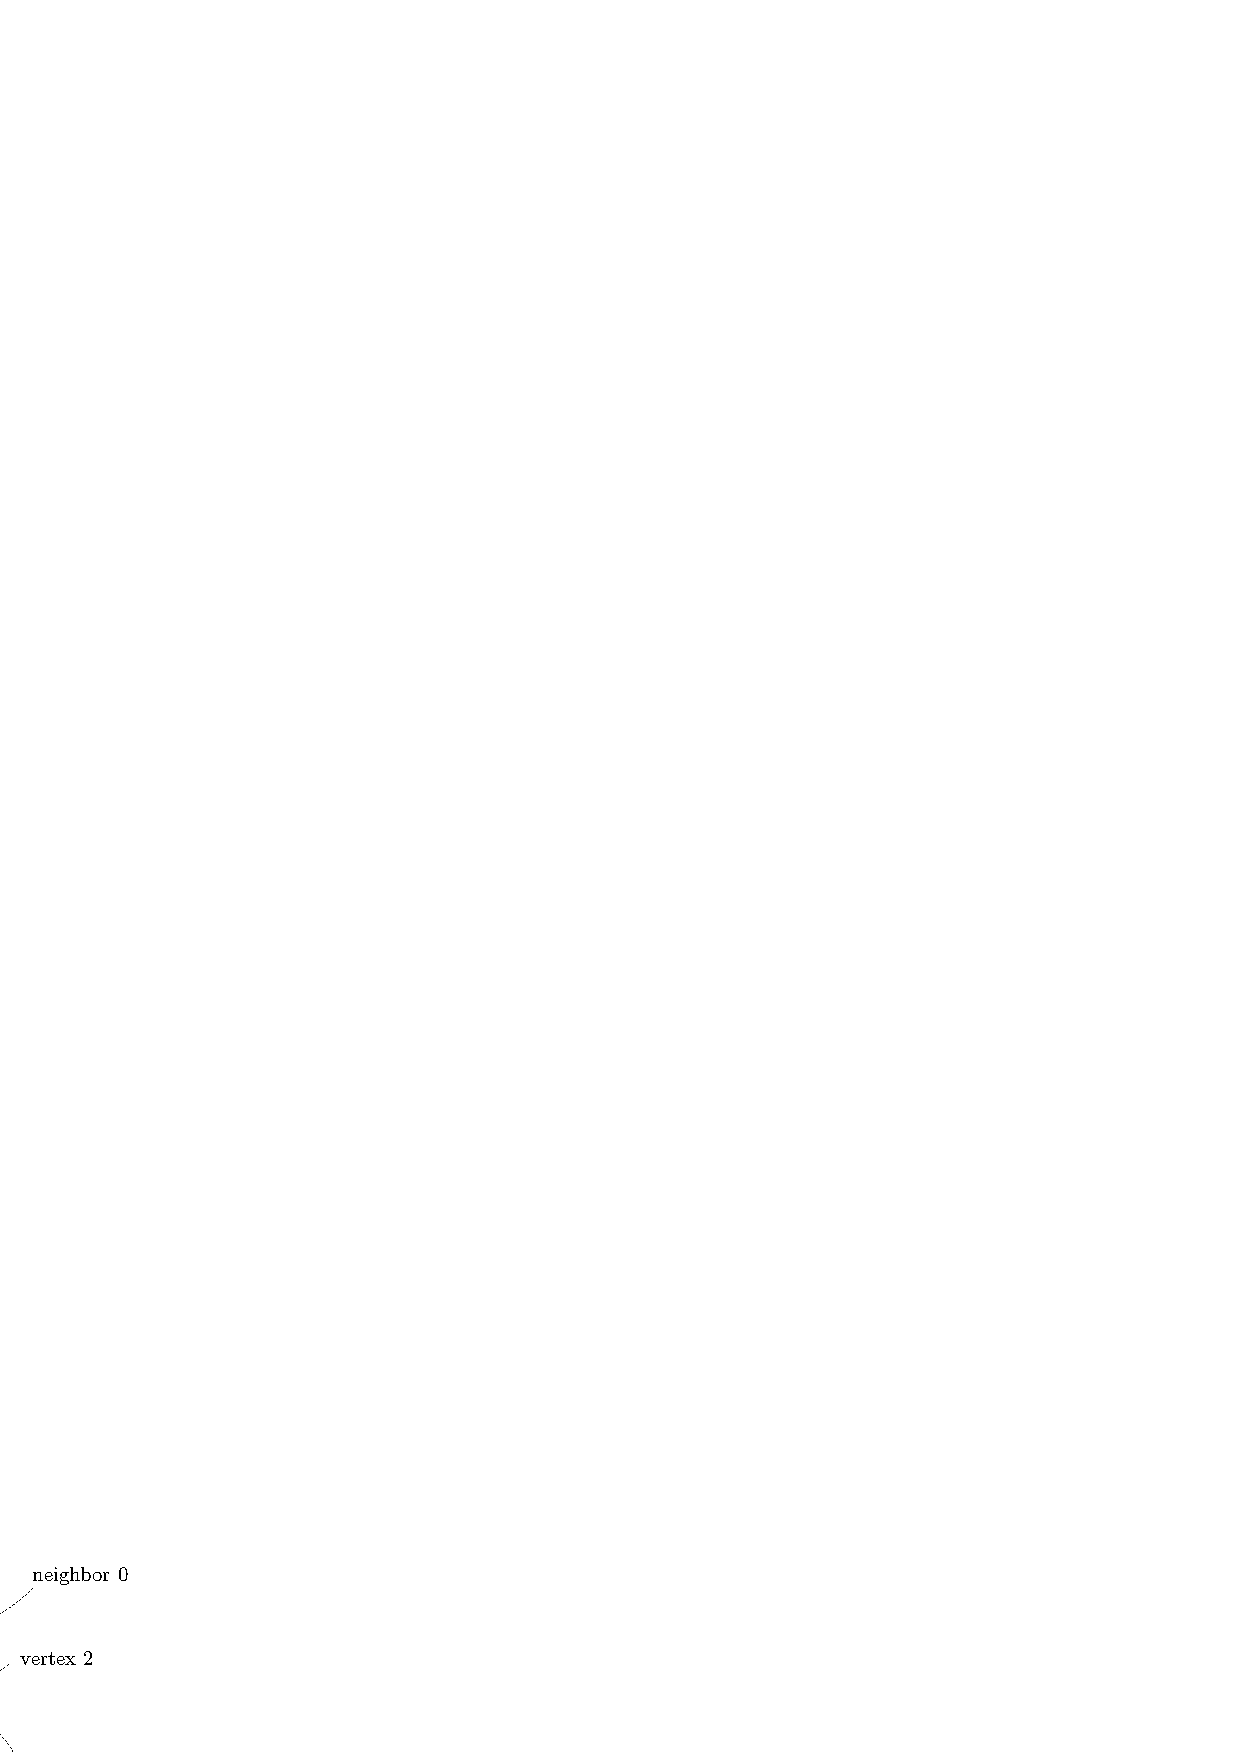
\includegraphics{TriangulationDS_3/repres}
\end{center}
\end{ccTexOnly}
\begin{ccHtmlOnly}
<CENTER>
<img border=0 src="./repres.gif" align=middle alt="Representation">
</CENTER>
\end{ccHtmlOnly}
\caption{Representation.
\label{TDS3-fig-repres}}
\end{figure} 

Edges ($1$-faces) and facets ($2$-faces) are not explicitly
represented: a facet is given by a cell and an index (the facet
\ccc{i} of a cell \ccc{c} is the facet of \ccc{c} that is opposite to
the vertex of index \ccc{i}) and an edge is given by a cell and two
indices (the edge \ccc{(i,j)} of a cell \ccc{c} is the edge
whose endpoints are the vertices of indices \ccc{i} and \ccc{j} of
\ccc{c}). 

\paragraph{Degenerate Dimensions}
As \cgal\ explicitly deals with all degenerate cases, a
3D-triangulation data structure in \cgal\ can handle the cases when
the dimension of the triangulation is lower than~3.

Thus, a 3D-triangulation data structure can store a triangulation of a
topological sphere $S^d$ of $\R^{d+1}$, for any $d \in \{-1,0,1,2,3\}$. 

Let us give, for each dimension, the example corresponding to the
triangulation data structure having a minimal number of vertices, i.e. a 
simplex. These examples are illustrated by presenting their usual
geometric embedding. 
\begin{itemize}
\item \emph{dimension 3.} The triangulation data structure consists of
the boundary of a 4-dimensional simplex, which has 5 vertices. A
geometric embedding consists in choosing one of these vertices to be
infinite, thus four of the five 3-cells become infinite: the geometric
triangulation has one finite tetrahedron remaining, each of its facets
being incident to an infinite cell. See Figure~\ref{TDS3-fig-topo-simplex4}.
\begin{figure}
\begin{ccTexOnly}
\begin{center} 
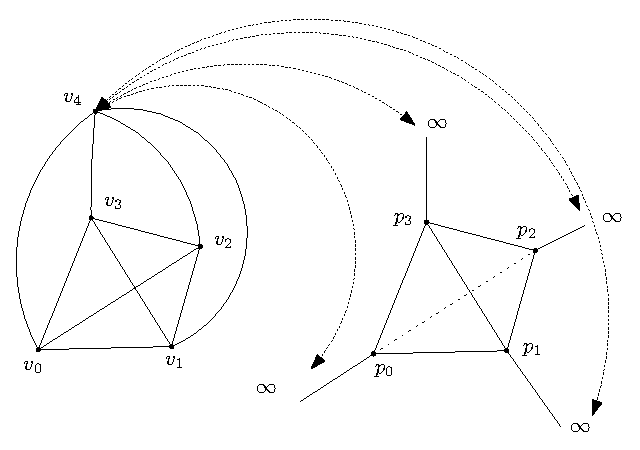
\includegraphics{TriangulationDS_3/topo-simplex4}
\end{center}
\end{ccTexOnly}
\begin{ccHtmlOnly}
<CENTER>
<img border=0 src="./topo-simplex4.gif" align=middle
alt="4D simplex and a 3D geometric embedding">
</CENTER>
\end{ccHtmlOnly}
\caption{4D simplex and a 3D geometric embedding.
\label{TDS3-fig-topo-simplex4}}
\end{figure} 
\item \emph{dimension 2.} We have 4 vertices forming one 3-dimensional
simplex, i.e. the boundary of a tetrahedron. The geometric embedding in
the plane results from choosing one of these vertices to be infinite,
then the geometric triangulation has one finite triangle whose edges are
incident to the infinite triangles. See Figure~\ref{TDS3-fig-topo-simplex3}.
\begin{figure}
\begin{ccTexOnly}
\begin{center} 
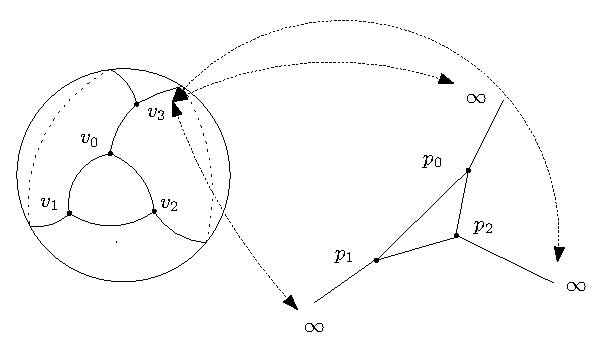
\includegraphics{TriangulationDS_3/topo-simplex3}
\end{center}
\end{ccTexOnly}
\begin{ccHtmlOnly}
<CENTER>
<img border=0 src="./topo-simplex3.gif" align=middle
alt="3D simplex and a 2D geometric embedding">
</CENTER>
\end{ccHtmlOnly}
\caption{3D simplex and a 2D geometric embedding.
\label{TDS3-fig-topo-simplex3}}
\end{figure} 
\item \emph{dimension 1.} A 2-dimensional simplex (a triangle) has 3
vertices. The geometric embedding is an edge whose vertices are linked
to an infinite point.  See Figure~\ref{TDS3-fig-topo-simplex2}.
\begin{figure}
\begin{ccTexOnly}
\begin{center} 
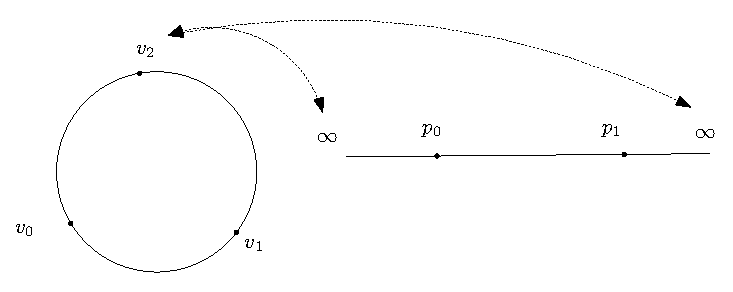
\includegraphics{TriangulationDS_3/topo-simplex2}
\end{center}
\end{ccTexOnly}
\begin{ccHtmlOnly}
<CENTER>
<img border=0 src="./topo-simplex2.gif" align=middle
alt="2D simplex and a 1D geometric embedding">
</CENTER>
\end{ccHtmlOnly}
\caption{2D simplex and a 1D geometric embedding.
\label{TDS3-fig-topo-simplex2}}
\end{figure} 
\end{itemize}

The last three cases are defined uniquely:
\begin{itemize}
\item \emph{dimension 0.} A 0-dimensional triangulation is
combinatorially equivalent to the boundary of a 1-dimensional simplex
(an edge), which consists of 2 vertices. One of them becomes infinite
in the geometric embedding, and there is only one finite vertex
remaining. The two vertices are adjacent.
\item \emph{dimension -1.} This dimension is a convention to represent a 
0-dimensional simplex, that is a sole vertex, which will be
geometrically embedded as an ``empty'' triangulation, having only one
infinite vertex.
\item \emph{dimension -2.} This is also a convention. The
triangulation data structure has no vertex. There is no associated
geometric triangulation.
\end{itemize} 

Note that the notion of infinite vertex has no meaning for the
triangulation data structure. The infinite vertex of the geometric
embedding is a vertex that cannot be distinguished from the other
vertices in the combinatorial triangulation.

The same cell class is used in all cases: triangular faces in
2D can be considered as degenerate cells, having only three vertices
(resp. neighbors) numbered $(0,1,2)$;
edges in 1D have only two vertices (resp. neighbors) numbered $0$ and $1$.

The implicit representation of facets (resp. edges) still holds
for degenerate ($< 3$) dimensions : in dimension~2, each cell has only one
facet of index 3, and 3 edges $(0,1)$, $(1,2)$ and $(2,0)$; in
dimension~1, each cell has one edge $(0,1)$. 

\paragraph{Validity}
A 3D combinatorial triangulation is said to be \ccc{locally valid} 
iff the following is true:

{\bf (a)} When a cell $c$ has a neighbor pointer to another cell $c'$,
then reciprocally this cell $c'$ has a neighbor pointer to $c$, and
$c$ and $c'$ have three vertices in common. These cells are called
adjacent. 
% Two adjacent cells have reciprocal neighbor pointers to each
% other and they have three vertices in common. 

{\bf (b)} The cells have a coherent orientation: if two cells $c_1$
and $c_2$ are adjacent and share a facet with vertices $u,v,w$, then
the vertices of $c_1$ are numbered $(v_0^1 = u, v_1^1 = v, v_2^1 = w,
v_3^1)$, and the vertices of $c_2$ are numbered $(v_0^2 = v, v_1^2 = u,
v_2^2 = w, v_3^2)$, up to positive permutations of $(0,1,2,3)$. In
other words, if we embed the triangulation in $\R^3$, then the fourth
vertices $v_3^1$ and $v_3^2$ of $c_1$ and $c_2$ see the common facet
in opposite orientations. See Figure~\ref{TDS3-fig-comborient}.

The set {\Large $\sigma$}$_4$ of permutations of
$(0,1,2,3)$ has cardinality 24, and the set of positive permutations
$A_4$ has cardinality 12. Thus, for a given orientation, there
are up to 12 different orderings of the four vertices of a cell. Note
that cyclic permutations are negative and so do not preserve the
orientation of a cell.

\begin{figure}[htbp]
\begin{ccTexOnly}
\begin{center} 
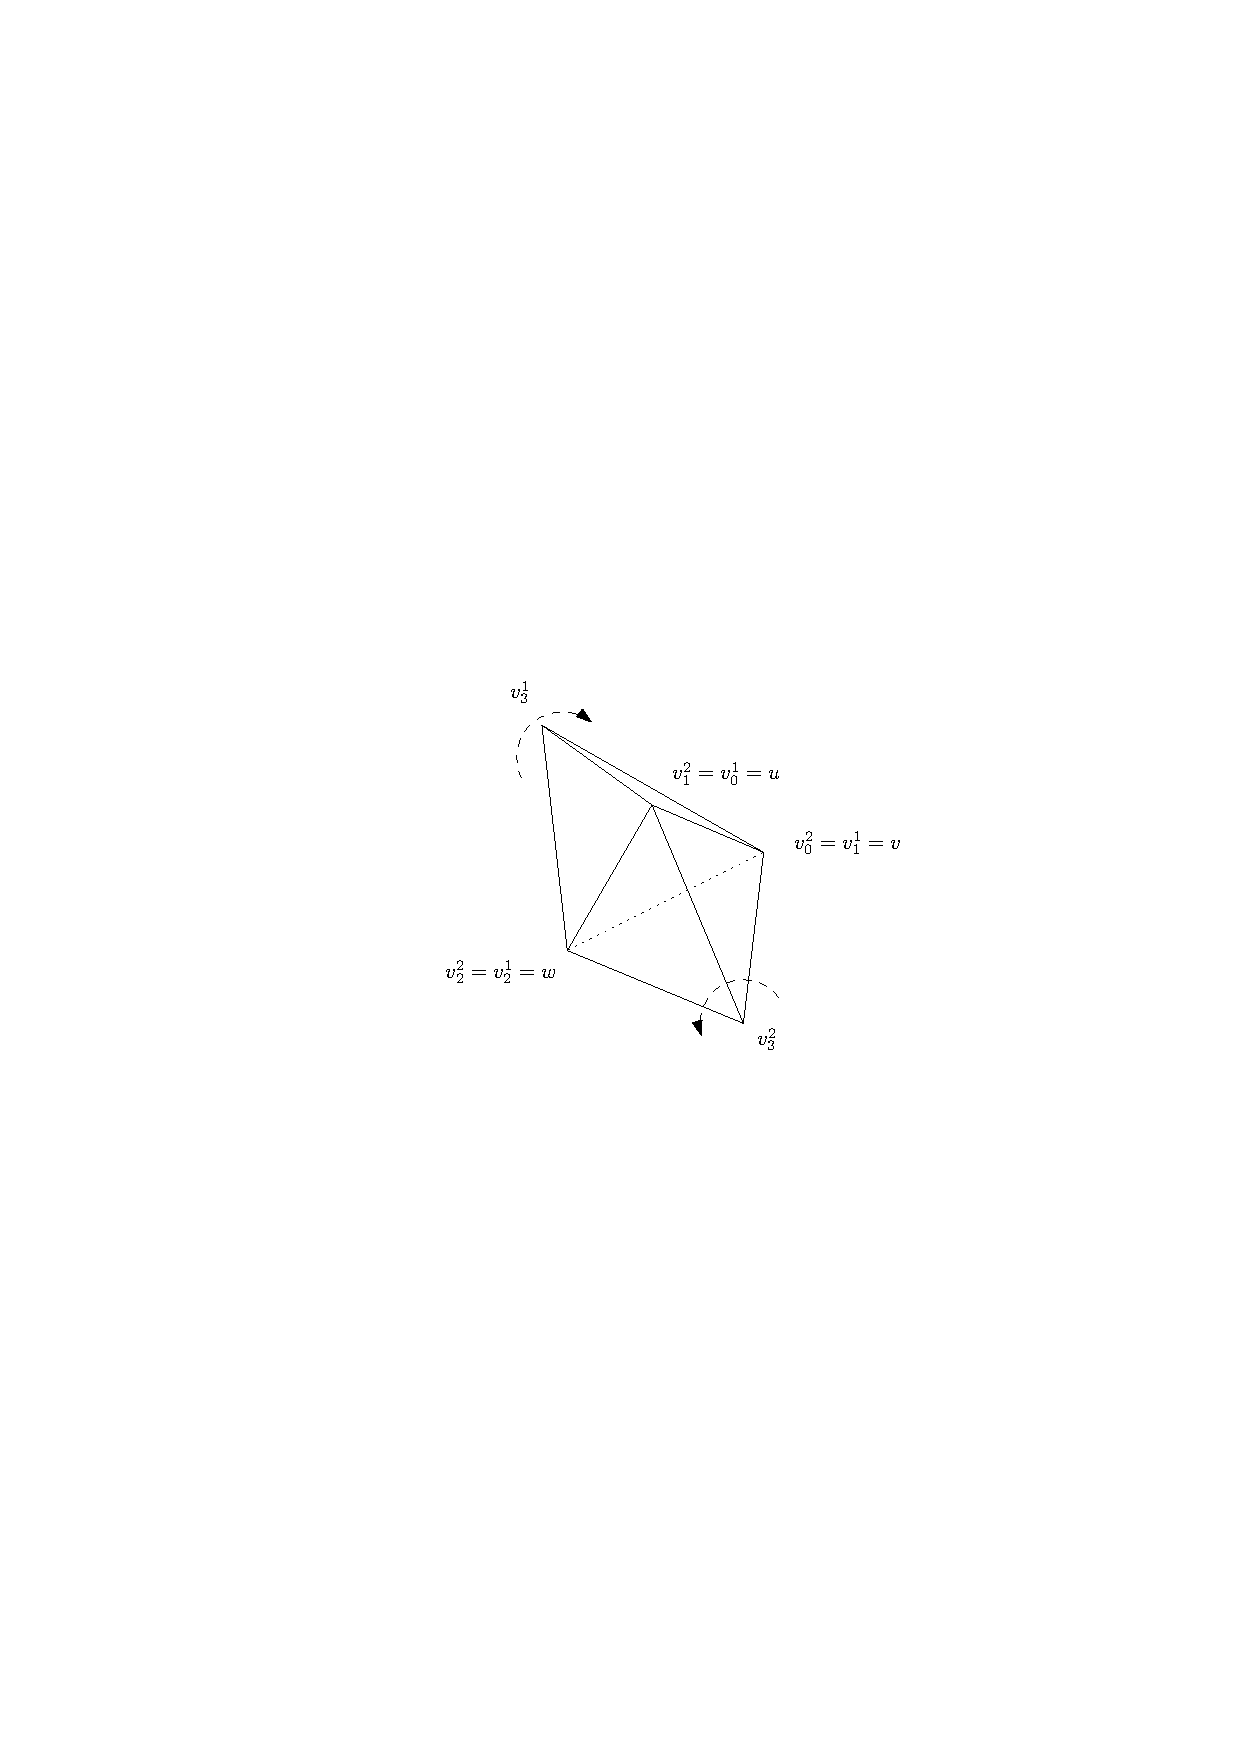
\includegraphics{TriangulationDS_3/comborient} 
\end{center}
\end{ccTexOnly}
\begin{ccHtmlOnly}
<CENTER>
<img border=0 src="./comborient.gif" align=middle alt="Orientation of a cell (3-dimensional case)">
</CENTER>
\end{ccHtmlOnly}
\caption{Coherent orientations of two cells (3-dimensional case).
\label{TDS3-fig-comborient}}
\end{figure} 

The \ccc{is_valid()} method provided by
\ccc{Triangulation_data_structure_3} checks the local validity of a
given triangulation data structure.
 
\section{Software Design\label{TDS3-sec-design}}

The 3D-triangulation data structure class of \cgal,
\ccc{Triangulation_data_structure_3}, is designed to be used as a combinatorial
layer upon which a geometric layer can be built \cite{k-ddsps-98}. This
geometric layer is typically one of the 3D-triangulation classes of \cgal:
\ccc{Triangulation_3}, \ccc{Delaunay_triangulation_3} and
\ccc{Regular_triangulation_3}. This relation is described in more details in
Chapter~\ref{chapter-Triangulation3}, where the
Section~\ref{Triangulation3-sec-design} explains other important parts of the
design related to the geometry.

We focus here on the design of the triangulation data structure (TDS)
itself, which the Figure~\ref{TDS3-fig-layers} illustrates.

\begin{figure}[htbp]
\begin{ccTexOnly}
\begin{center}
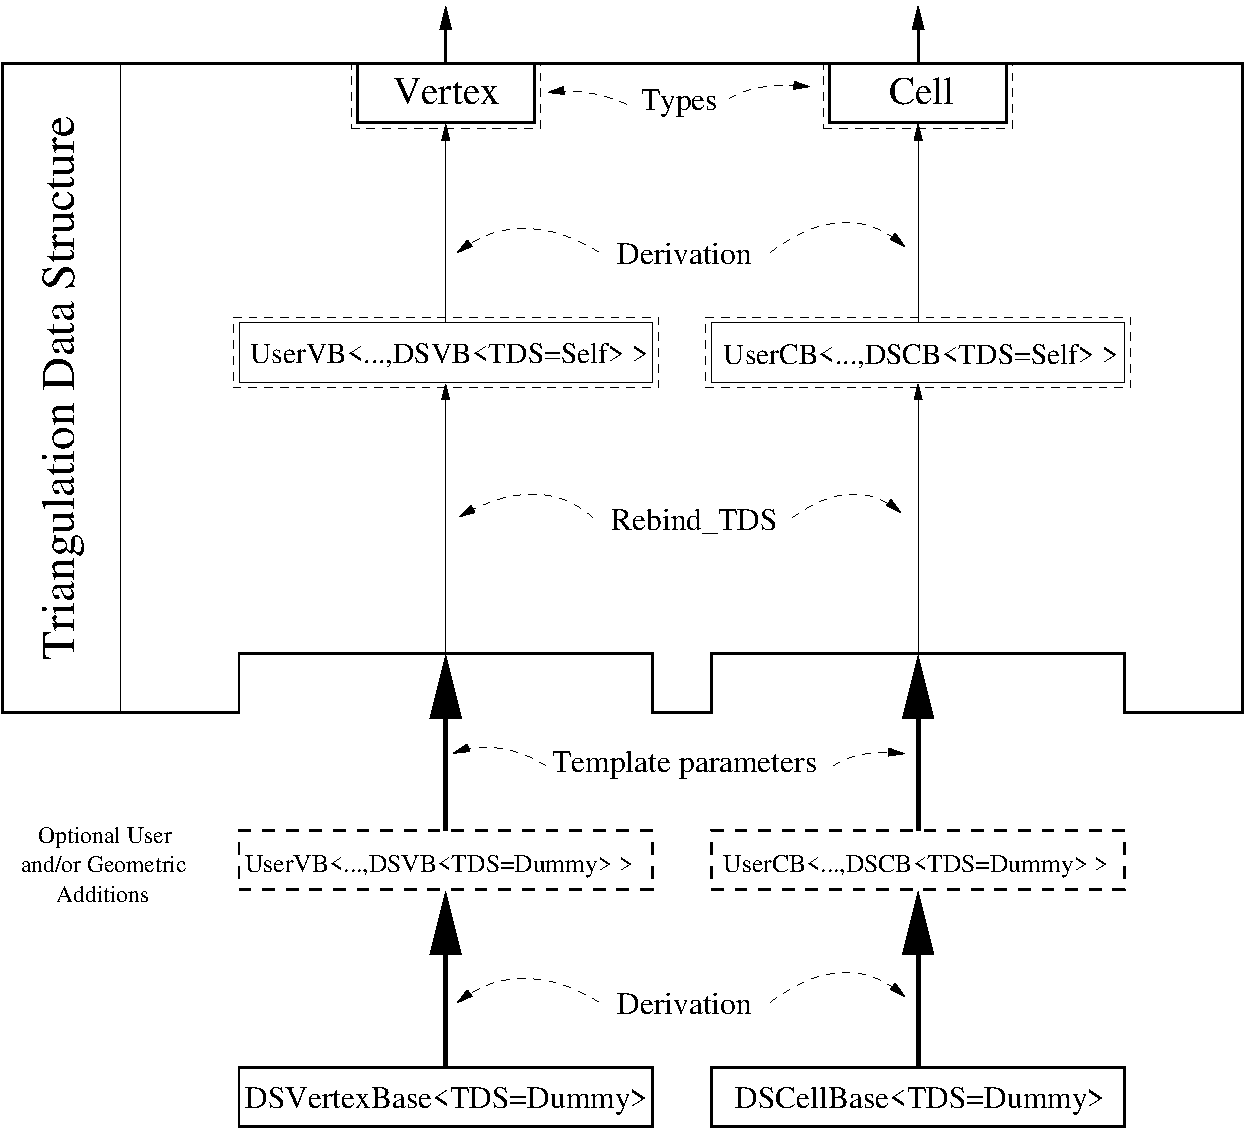
\includegraphics[width=14cm]{TriangulationDS_3/design_tds}
\end{center}
\end{ccTexOnly}
\begin{ccHtmlOnly}
<CENTER>
<img border=0 src="./design_tds.gif" align=middle
 alt="Triangulation Data Structure software design">
</CENTER>
\end{ccHtmlOnly}
\caption{Triangulation Data Structure software design.
\label{TDS3-fig-layers}}
\end{figure} 

\subsection{Flexibility of the Design}

In order for the user to be able to add his own data in the vertices and cells,
the design of the TDS is split into two layers:

\begin{itemize}
\item{} In the bottom layer, the (vertex and cell) base classes store
elementary incidence and adjacency (and possibly geometric or other)
information.  These classes are parameterized by the TDS which provides the
handle types.  (They can also be parameterized by a geometric traits class or
anything else.) A vertex stores a \ccc{Cell_handle}, and a cell stores four
\ccc{Vertex_handle}s and four \ccc{Cell_handle}s.

\item{} The middle layer is the TDS, which is purely combinatorial.  It
provides operations such as insertion of a new vertex in a given cell, on a $1$
or $2$-face. It also allows one, if the dimension of the triangulation is
smaller than $3$, to insert a vertex so that the dimension of the triangulation
is increased by one. The TDS is responsible for the combinatorial integrity of
the eventual geometric triangulation built on top of it (the upper layer,
see Chapter~\ref{chapter-Triangulation3}).
\end{itemize}

The user has several ways to add his own data in the vertex and cell base classes used by the TDS.  He can either:
\begin{itemize}
\item{} use the classes \ccc{Triangulation_vertex_base_with_info_3}
and \ccc{Triangulation_cell_base_with_info_3}, which allow to add one data member
of a user provided type, and give access to it.
\item{} derive his own classes from the default base classes
\ccc{Triangulation_ds_vertex_base}, and \ccc{Triangulation_ds_cell_base} (or
the geometric versions typically used by the geometric layer,
\ccc{Triangulation_vertex_base}, and \ccc{Triangulation_cell_base}).
\item{} write his own base classes following the requirements given by the
concepts \ccc{TriangulationCellBase_3} and \ccc{TriangulationVertexBase_3}
\lcTex{(described in \ccRefPage{TriangulationCellBase_3} and
\ccRefPage{TriangulationVertexBase_3})}.
\end{itemize}

\subsection{Cyclic Dependency\label{tds3-cyclic}}

Since adjacency relations are stored in the vertices and cells, it means that
the vertex and cell base classes have to be able to store handles (an entity
akin to pointers) to their neighbors in the TDS.  This in turns means that the
vertex and cell base classes have to know the types of these handles, which are
provided by the TDS.  So in a sense, the base classes are parameterized by the
TDS, and the TDS is parameterized by the vertex and cell base classes !
This is a cycle which cannot be resolved easily.

The solution that we have chosen is similar to the mechanism used by the
standard class \ccc{std::allocator}: the vertex and cell base classes are
initially given a fake or dummy TDS template parameter, whose unique purpose
is to provide the types that can be used by the vertex and cell base classes
(such as handles).  Then, inside the TDS itself, these base classes are
\textit{rebound} to the real TDS type, that is we obtain the same vertex
and cell base classes, but parameterized with the real TDS instead of the dummy
one.  Rebinding is performed by a nested template class of the vertex and cell
base classes (see code below), which provides a type which is the rebound
vertex or cell base class\footnote{It is logically equivalent to a mechanism
that does not exist yet in the C++ language: \textit{template typedef} or
\textit{template aliasing}}.

Here is how it works, schematically:

\begin{ccExampleCode}
template < class Vb, class Cb >
class TDS
{
  typedef TDS<Vb, Cb>    Self;

  // Rebind the vertex and cell base to the actual TDS (Self).
  typedef typename Vb::template Rebind_TDS<Self>::Other  VertexBase;
  typedef typename Cb::template Rebind_TDS<Self>::Other  CellBase;

  // ... further internal machinery leads to the final public types:
public:
  typedef ...  Vertex;
  typedef ...  Cell;
  typedef ...  Vertex_handle;
  typedef ...  Cell_handle;
};

template < class TDS = ... >  // The default is some internal type faking a TDS
class Triangulation_ds_vertex_base_3
{
public:
  template < class TDS2 >
  struct Rebind_TDS {
    typedef Triangulation_ds_vertex_base_3<TDS2>    Other;
  };
...
};
\end{ccExampleCode}

When derivation is used for the vertex or cell base classes, which is the
case at the geometric level with \ccc{Triangulation_vertex_base_3}, then
it gets slightly more involved because its base class has to be rebound as
well:

\begin{ccExampleCode}
template < class GT, class Vb = Triangulation_ds_vertex_base_3<> >
class Triangulation_vertex_base_3 : public Vb
{
public:
  template < class TDS2 >
  struct Rebind_TDS {
    typedef typename Vb::template Rebind_TDS<TDS2>::Other  Vb2;
    typedef Triangulation_vertex_base_3<GT, Vb2>           Other;
  };
...
};
\end{ccExampleCode}

\section{Examples\label{TDS3-sec-examples}}

\subsection{Incremental Construction}
The following example shows how to construct a 3D triangulation data
structure by inserting vertices.

\ccIncludeExampleCode{Triangulation_3/tds.cpp}

\subsection{Cross-Linking Between a 2D and a 3D Data Structures}
This example program illustrates how to setup a 2D and a 3D triangulation data
structures whose vertices respectively store vertex handles of the other one.

\ccIncludeExampleCode{Triangulation_3/linking_2d_and_3d.cpp}

%%%%%%%%%%%%%%%%%%%%%%%%%%%%%%%%
\section{Design and Implementation History}

Monique Teillaud introduced the triangulation of the topological
sphere $S^d$ in $\R^{d+1}$ to manage the underlying graph of geometric
triangulations and handle degenerate dimensions \cite{t-tdtc-99}. 

Sylvain Pion improved the software in several ways, in particular
regarding the memory management.
